\documentclass{bfh}

\usepackage[numbers]{natbib}
\usepackage{xfrac}

\title{Informatikseminar}
\subtitle{Bitmessage -- Communication Without Metadata}
\author{Christian Basler}
\tutor{Kai Brünnler}
\date{\today}

\newcommand{\msg}[1]{\textit{\textcolor{RedOrange}{#1}}}
\newcommand{\obj}[1]{\textbf{\textcolor{OliveGreen}{#1}}}
\newcommand{\node}[1]{\textbf{\textcolor{MidnightBlue}{#1}}}

\begin{document}
  \maketitle

  \tableofcontents

  \listoffigures

  \newpage
  \section*{Abstract}

  Even if we use encryption, we reveal a lot about ourselves in the metadata we produce. Bitmessage prevents this by distributing a message in a way that it's not possible to find out which was the intended recipient.

  \newpage
  % Section basics
    \section{Basics}

  While encryption technology like PGP or S/MIME provides a secure way to protect content from prying eyes, we lerned from Edward Snowden that metadata - information about who communicates with whom - is equally interesting and much easier to analyze.

  With e-mail, we can only prevent this by encrypting the connection to the server as well as between servers. Therefore we can only hope that both our and the recipient's e-mail provider are both trustworthy and competent.

  With Bitmessage we send a message to a sufficiently large number of participants, with the intended recipient among them. The message is encrypted such as only the person in possesion of the private key can decrypt it. All participants try to do this in order to find their messages.


  \newpage
  \section{Protocol}

  We use the following convention to distinguish different parts of the protocol:

  \begin{tabular}{@{}>{$}l<{$}l@{}}
	\msg{version} & for messages between nodes \\
	\obj{pubkey} & for objects that are spread throughout the network \\
	\node{A} & for individual nodes \\
  \end{tabular}


  \subsection{Nomenclature}

  There are a few terms that are easily mixed up. Here's a list of the most confusing ones:

  \subsubsection{message, msg}
  A \msg{message} is sent from one node to another, i.e. to announce new objects or to initialize the network connection.

  An \obj{msg} on the other hand is the object payload containing content written by a user.

  In the protocol section, the term 'message' is never used to describe information exchange between users.

  \subsubsection{payload}
  There are three kinds of payload:
  \begin{enumerate}
  \item Message payload for message types, e.g. containing inventory vectors.
  \item Object payload, which is distributed throughout the network.\footnote{And part of the message payload.}
  \item Encrypted payload, which is the ciphertext with some metadata needed for decryption.\footnote{Which, again, is part of the object payload.}
  \end{enumerate}

  \subsubsection{object}
  An object is a kind of message whose payload is distributed among all nodes. Somtimes just the payload is meant. To send an object, proof of work is required.

  \subsection{Process Flow}

  The newly started node \node{A} connects to a random node \node{B} from its node registry and sends a \msg{version} message, announcing the latest supported protocol version. If \node{B} accepts the version,\footnote{A version is accepted by default if it is higher or equal to a nodes latest supported version. Nodes supporting experimental protocol versions might accept older versions.} it responds with a \msg{verack} message, followed by a \msg{version} message announcing its own latest supported protocol version. Node \node{A} then decides whether it supports \node{B}'s version and sends its \msg{verack} message.

  If both nodes accept the connection, they both send an \msg{addr} message containing up to 1000 of its known nodes, followed by one or more \msg{inv} messages announcing all valid objects they are aware of. They then send \msg{getobject} request for all objects still missing from their inventory.

  \msg{Getobject} requests are answered by \msg{object} messages containing the requested objects.

  A node actively connects to eight other nodes, allowing any number of incoming connections. If a user creates a new object on node \node{A}, it is offered via \msg{inv} to eight of the connected nodes. They will get the object and distribute it to up to eight of their connections, and so on, until all nodes have it in their inventory.

  \subsection{Messages}

  The messages, objects and binary format are very well discribed in the Bitmessage wiki \cite{wiki:protocol}, the message description is therefore narrowed down to a description of what they do and when they're used.

  \subsubsection{version / verack}
  A \msg{version} message contains the latest protocol version supported by a node, as well as the streams it is interested in and which features it supports. If the other node accepts, it acknowledges with a \msg{verack} message. The connection is initialized when both nodes sent a \msg{verack} message.

  \subsubsection{addr}
  Contains up to 1000 known nodes with their IP addresses, ports, streams and supported features.

  \subsubsection{inv}
  One \msg{inv} message contains the hashes of up to 50000 valid objects. If your inventory is larger, several messages can be sent.

  \subsubsection{getdata}
  Can request up to 50000 objects by sending their hashes.

  \subsubsection{object}
  Contains one requested object, which might be one of:

  \listinginfo{}{getpubkey}{A request for a public key, which is needed to encrypt a message to a specific user.}{}
  \listinginfo{}{pubkey}{A public key. See \ref{subsec:addr} \nameref{subsec:addr}}{}
  \listinginfo{}{msg}{Content intended to be received by one user.}{}
  \listinginfo{}{broadcast}{Content sent in a way that the Addresses public key can be used to decrypt it, allowing any subscriber who knows the address to receive the such a message}{}

  \subsubsection{ping / pong / getbiginv}
  People looking at the PyBitmessage's source code might be irritated by some other messages that seem to be implemented, but aren't mentioned in the official protocol specification. \msg{ping} does actually cause the node that implements this to send a \msg{pong} message, but this feature isn't actually used anywhere. \msg{getbiginv} seems to be thought for requesting the inventory, but as I understand it can't be used. \cite{issue:112}

  \subsection{Addresses}
  \label{subsec:addr}

  \textit{BM-2cXxfcSetKnbHJX2Y85rSkaVpsdNUZ5q9h}: Addresses start with "BM-" and are, like Bitcoin addresses, Base58 encoded.\footnote{Which uses characters 1-9, A-Z and a-z without the easily confused characters I, l, 0 and O.}

  \listinginfo{}{version}{Address version.}{}
  \listinginfo{}{stream}{Stream number.}{}
  \listinginfo{}{ripe}{Hash of both public signing and encryption key. Please note that the keys are sent without the leading 0x04 in \obj{pubkey} objects, but for creating the ripe it must be prepended. This is also necessary for most other applications, so it's a good idea to do it by default.}{ripemd160(sha512(pubSigKey + pubEncKey))}
  \listinginfo{}{checksum}{First four bytes of a double SHA-512 hash of the above.}{sha512(sha512(version + stream + ripe))}

  \subsection{Encryption}

  Bitmessage uses Elliptic Curve Cryptography for both signing and encryption. While the mathematics behind elliptic curves is even harder to understand than the older approach of multiplying huge primes, it's based on the same principle of doing some mathematical operation that can be done fast one way but is very hard to reverse. Instead of two very large primes, we multiply a point on the elliptic curve by a very large number.\footnote{Please don't ask me how to do it. If you really want to know, start at \url{http://en.wikipedia.org/wiki/Elliptic_curve_point_multiplication} and \url{http://en.wikipedia.org/wiki/Elliptic_curve_cryptography}. If you want to make something that works, use a library like Bouncy Casle that does the heavy lifting for you.}

  The user, let's call her Alice, needs a key pair, consisting of a private key
$$k$$
which represents a huge random number, and a public key
$$K = G k$$
which represents a point on the agreed on curve.\footnote{Bitmessage uses a curve called \textit{secp256k1}.} Please note that this is not a simple multiplication, but the multiplication of a point along an elliptic curve. $G$ is the starting point for all operations on a specific curve.

  Another user, Bob, knows the public key. To encrypt a message, Bob creates a temporary key pair
$$r$$
and
$$R = G r$$
He then calculates
$$K r$$
uses the resulting Point to encrypt the message\footnote{A double SHA-512 hash over the x-coordinate is used to create the actual key.} and sends $K$ along with the message.

  When Alice receives the message, she uses the fact that
$$K r = G k r = G r k = R k$$
so she just uses $R k$ to decrypt the message.

  The exact method used in Bitmessage is called Elliptic Curve Integrated Encryption Scheme or ECIES, which is described in detail on Wikipedia (\url{http://en.wikipedia.org/wiki/Integrated_Encryption_Scheme}).

  \subsubsection{Signature}

  To sign objects, Bitmessage uses Elliptic Curve Digital Signature Algorithm or ECDSA. This is slightly more complicated, if you want the details, Wikipedia is once again a fine starting point: \url{http://en.wikipedia.org/wiki/Elliptic_Curve_Digital_Signature_Algorithm}.

  A detail that's interesting for people who want to implement a Bitmessage client, particularly if they do it using some object oriented approach: the signature covers everything from the object header sans nonce, and everything from the object payload except for the signature itself. Of course, not all objects are signed.\footnote{My approach was: think first, do it wrong, then refactor a lot.}

  \newpage
  \section{Issues}

  \subsection{Scalability}

  Bitmessage doen't scale.\footnote{Yet.} If there are very few users, anonymity isn't given anymore. With just a handful users, it's easy (for, let's say the NSA) to analyse traffic between nodes to find out who they might be writing to. Or let's just put them all under surveilance.

  With many users, traffic and storage use grows quadratically. This, because with more users there are more people who write messages as well as more users to write to for existing users.

  \subsubsection{Proof of Work}
  Proof of work has two uses. It helps to protect the network by preventing single nodes from flooding it with objects, and to protect users from spam. There's minimal proof of work required for the network to distribute objects, but users can define higher requirements for their addresses if they get spammed with cheap Viagra\texttrademark{} offers. The proof of work required for an address is defined in the \obj{pubkey}, and senders that are in a user's contacts should not be required to do the higher proof of work.

  The difficulty is calculated from both message size as well as time to live, meaning that a message that is larger or stored longer in the network will be more expensive to send.
$$ d = \frac{2^{64}}{n (l + \frac{t l}{2^{16}})} $$
\begin{tabular}{@{}>{$}l<{$}l@{}}
	d & target difficulty \\
	n & required trials per byte \\
	l & payload length + extra bytes (in order to not make it too easy to send a lot of tiny messages) \\
	t & time to live \\
\end{tabular}

  To do the proof of work, a nonce must be found such that the first eight bytes of the hash of the object (including the nonce) represent a lower number than the target difficulty.

  \subsubsection{Message Size Limitation}
  To prevent malicious users from clogging individual nodes, messages must not be larger than 256 KiB. Because of the proof of work, large objects arent' practical for normal use, but might be used to occupy nodes by sending them garbage.

  \subsubsection{Streams}
  The intended solution for this problem is splitting traffic -- addresses, more precisely -- into streams. A node listens only on the streams that concern its addresses. If it wants to send an object to another stream, it just connects to a node in this stream to send the object, then disconnects. When all active streams are full, a new one is created which should be used for new addresses.

  The unsolved problem is to determine when a stream is full. Another issue is the fact that, as the overall network grows, traffic on full streams still grows, as there are more users who might wanto to write someone on the full stream.

  \subsubsection{Prefix Filtering}
  Jonathan Coe proposed this interesting way of handling traffic. This would need an update to the protocol, but allows for much finer grained control of how much traffic a node wants to handle.\cite{wiki:prefixfilter}

  Instead of streams, we imagine an address as a leave of a binary tree of height 65. The position is defined by the first 64 bits of the address' ripe. A prefix value $n$ defines the node at wich we start to listen. A client sending a message sets a 64 bit nonce where the first $n$ bits are copied from the recipient's ripe, and the rest is set randomly.

  \begin{figure}[htp]
  \centering
  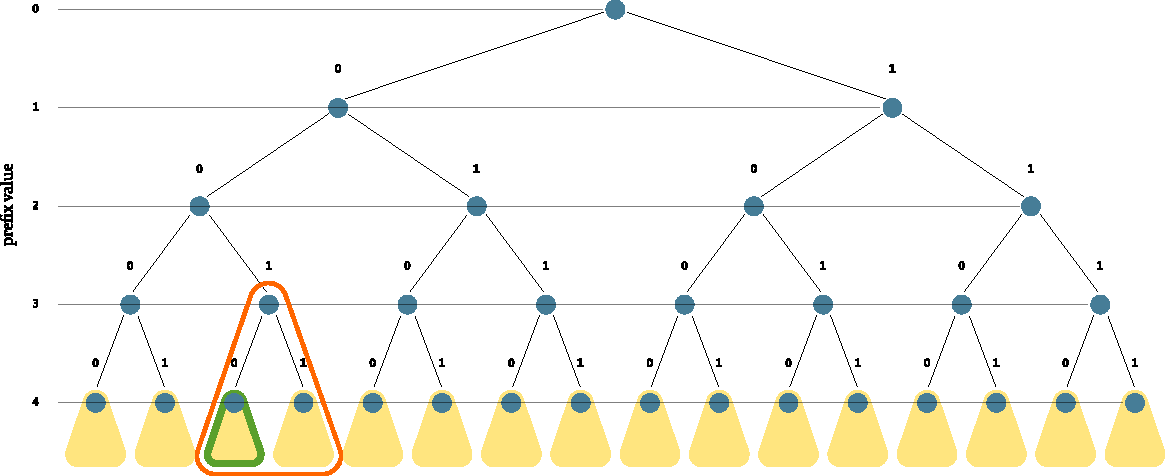
\includegraphics[width=\textwidth]{images/prefix-filter-binary-tree.pdf}
  \caption[prefix filter: binary tree]{Note that the prefix value goes up to 64, i.e. each yellow triangle is itself a subtree of height 61.}
  \label{fig:bintree}
  \end{figure}

  Now let's assume Bob's address' ripe starts with \texttt{00101001\ldots} and his prefix value is 3. Alice sends a message tagged with \texttt{00110100\ldots}. The first three bits must be the same, but the rest is random. Bob's client now gets only objects that match his prefix, meaning he must only handle \sfrac{1}{8} of the overall traffic.\footnote{At the moment, the overall traffic is around 1 GiB per month.}

  As Bitmessage might get more popular, it would produce more and more traffic. Bob therefore might want to raise his prefix value to 4, further reducing the traffic he handles to \sfrac{1}{16} of the overall traffic. To do this, he simply publishes his \obj{pubkey} with the updated prefix value. This means of course that either must there always be a pubkey published, or Alice needs to be online at least once while the pubkey is published. Otherwise there's a 50\% chance (in our scenario) that the message won't reach Bob.

  While this would allow for a mobile client to only process messages meant for its addresses,\footnote{Choosing a prefix value of 64 would most certainly mean that it's alone on this stream.} this would mean to give up anonymity almost completely.

  TODO

  .

  .

  .

  .

  .

  .

  \subsection{Forward Secrecy}

  Obviously it's trivial for an attacker to collect all (encrypted) objects distributed through the Bitmessage network -- as long as disk space is not an issue. If this attacker can somehow get the private key of a user, they can decrypt all stored messages intended for that user, as well as impersonate said user.\footnote{The latter might be more difficult if they got the key through a brute force attack.}

  Plausible deniability can, in some scenarios, help against this. This action, called "nuking an address", is done by anonymously publishing the private keys somewhere publicly accessible.\footnote{See \url{https://bitmessage.ch/nuked/} for an example.}

  Perfect forward secrecy seems impractical to implement, as it requires to exchange messages prior to sending encrypted content. That would in turn need proof of work to protect the network, resulting in twice the work for the sender and three times longer to send --- that is, if both clients are online. Exchanging messages would be all but impossible if both users are online sporadically.

  \newpage
  \section{Discussion}

  Anonymity has its price. With Bitmessage it's traffic and disk space, with E-Mail it's trust. If we can't trust our e-mail providers (who can?), Bitmessage is a very interesting alternative, albeit not fully matured.

  TODO

  .

  .

  .

  .

  .

  .


  \bibliographystyle{plain}
  \bibliography{bibliography}

  \appendix
  \addcontentsline{toc}{section}{Appendix}
  \section*{Appendix}
  \renewcommand{\thesubsection}{\Alph{subsection}}

  \subsection{TODO}

\end{document}